\documentclass{article}
\usepackage[utf8]{inputenc}
\usepackage{amsmath}
\usepackage{authblk}
\usepackage{graphicx}
\usepackage{caption}
\usepackage{subcaption}
\usepackage[portuguese]{babel}
\usepackage{csquotes}
\usepackage{multicol}

\usepackage[sorting=none]{biblatex}
\addbibresource{bib.bib}

\title{Localização Probabilística de Robôs com Redundância de Faróis}
\author[1]{João Santos, 76912}
\affil[1]{Departamento de Eletrónica, Telecomunicações e Informática, Universidade de Aveiro}
\date{Maio 2022}

\begin{document}

\maketitle

\section{Introdução}

Para navegar eficazmente e atingir objetivos, os robôs móveis devem ser capazes de determinar a sua posição em relação a locais conhecidos no ambiente. Esta é a problemática da localização.

O \textit{dead-reckoning} é o método mais básico para a tentar realizar\cite{833191}. Este método utiliza o histórico de velocidades do robô ao longo do tempo para calcular a mudança de posição a partir do ponto de partida. Infelizmente, os métodos de cálculo de \textit{dead-reckoning} puro são propensos a erros que crescem continuamente ao longo do tempo, exigindo a utilização de um segundo método de correção numa base regular. Técnicas adicionais de localização, tais como triangulação de pontos de referência ou correspondência de mapas, são frequentemente combinadas com o \textit{dead-reckoning}, utilizando um filtro Kalman estendido para atualizar probabilisticamente a posição do robô.

\section{Metodologia}

Num ambiente 2D composto por vários faróis com posições conhecidas, tem-se como objetivo que o robô móvel visite, por ordem, todos os faróis, parando no último, percorrendo uma trajetória suave tentando sempre manter uma estimativa da sua pose atual.

Paralelamente, existe a necessidade de verificar que as velocidades a impor ao robô são fisicamente possíveis, recorrendo à cinemática inversa de três modelos móveis.

Este projeto recorreu intensivamente à libraria \textit{SymPy}\cite{sympy} para o cálculo simbólico. Várias equações intermédias foram omitidas.

\subsection{Filtro de Kalman Estendido}

Em 1960, Rudolf Kálmán publicou um artigo\cite{kalman1960} em que descrevia uma solução recursiva ao problema da filtragem linear de dados discretos. O filtro de Kalman é um conjunto de equações matemáticas que proporcionam uma computação eficiente para estimar o estado de um processo, de forma a minimizar o erro quadrático médio.

Para casos em que o processo a ser estimado é não linear é frequentemente utilizado o filtro de Kalman estendido (EKF, do inglês) que lineariza em torno de média e da covariância.

Numa primeira instância, com base no estado atual do sistema $\hat{x}_k$, num dado controlo $u_k$ e no ruído associado $w_k$, este filtro tenta prever o estado futuro $\bar{x}_{k+1}$ e a respetiva covariância $\bar{P}_{k+1}$ (eq. \ref{eq:ekf_prediction}).

\begin{equation}
    \begin{cases}
        \bar{x}_{k+1} =& f(\hat{x}_k,u_k,w_k) \\
        \bar{P}_{k+1} =& J_{f_x}(\hat{x}_k,u_k,w_k) P_k J_{f_x}^T(\hat{x}_k,u_k,w_k) + \\
        &+J_{f_\omega}(\hat{x}_k,u_k,w_k) Q_k J_{f_\omega}^T(\hat{x}_k,u_k,w_k)
    \end{cases}
    \label{eq:ekf_prediction}
\end{equation}

De seguida, a inovação (i.e. é diferença entre as observações obtidos e as esperadas, para um dado estado) são usados em conjunto com o ganho de Kalman $K$ para produzir uma melhor estimativa do estado atual do sistema $\hat{x}_{k+1}$. A covariância do processo $P_{k+1}$ é também atualizada com recurso ao ganho de Kalman e à covariância da inovação $S$ (eq. \ref{eq:ekf_update}).

\begin{equation}
    \begin{cases}
        \hat{x}_{k+1} &= \bar{x}_{k+1} + K (z_{k+1} - h(\bar{x}_{k+1})) \\
        P_{k+1} &= \bar{P}_{k+1} - KSK^T \\
        S &= J_h(\bar{x}_{k+1}) \bar{P}_{k+1} J_h^T(\bar{x}_{k+1}) + R \\
        K &= \bar{P}_{k+1} J_h^T(\bar{x}_{k+1}) S^{-1}
    \end{cases}
    \label{eq:ekf_update}
\end{equation}

Para ser possível prever o estado futuro do sistema é necessária a existência de uma função de transição de estado $f$. No caso de um robô móvel, a eq. \ref{eq:motion_model} define o modelo cinemático genérico do mesmo, onde ao controlo de velocidade linear $V_k$ e angular $\omega_k$ são adicionados os respetivos ruídos gaussianos $\delta V_k$ e $\delta \omega_k$. Na etapa de previsão é convencional definir-se que $w_k = 0$. Como é também assumido que o intervalo de tempo $\Delta t$ é definido e constante, este é omitido nos parâmetros do modelo.

\begin{equation}
    \begin{split}
        f(\hat{x}_k,u_k,w_k) =&
        \begin{bmatrix}
        x_{k+1} \\
        y_{k+1} \\
        \theta_{k+1} 
        \end{bmatrix} 
        = \begin{bmatrix}
        x_k \\
        y_k \\
        \theta_k
        \end{bmatrix} + 
        \begin{bmatrix}
        \cos(\theta_k) & 0 \\
        \sin(\theta_k) & 0 \\
        0 & 1
        \end{bmatrix} \left(
        \begin{bmatrix}
        V_k \\
        \omega_k
        \end{bmatrix} + 
        \begin{bmatrix}
        \delta V_k \\
        \delta \omega_k
        \end{bmatrix}
        \right) \Delta t 
    \end{split}
    \label{eq:motion_model}
\end{equation}

Para a previsão da covariância são ainda necessários os Jacobianos da função $f$ relativamente ao vetor de estado $J_{f_x}$ e ao vetor de ruídos $J_{f_\omega}$, que estão definidos, respetivamente, nas equações \ref{eq:motion_model_jacobian_x} e \ref{eq:motion_model_jacobian_w}.

\begin{equation}
    J_{f_x}(\hat{x}_k,u_k,w_k) = \left[\begin{matrix}1 & 0 & - \Delta t \left(v_{k} + \delta V_k \right) \sin{\left(\theta_{k} \right)}\\0 & 1 & \Delta t \left(v_{k} + \delta V_k \right) \cos{\left(\theta_{k} \right)}\\0 & 0 & 1\end{matrix}\right]
    \label{eq:motion_model_jacobian_x}
\end{equation}

\begin{equation}
    J_{f_\omega}(\hat{x}_k,u_k) = \left[\begin{matrix}\Delta t \cos{\left(\theta_{k} \right)} & 0\\ \Delta t \sin{\left(\theta_{k} \right)} & 0\\0 & \Delta t\end{matrix}\right]
    \label{eq:motion_model_jacobian_w}
\end{equation}

Já na etapa de atualização, um dos requisitos do filtro de Kalman é que seja possível computacional as medições esperados dos sensores para um determinado estado. No caso particular em que os sensores detetam a distância $r^i$ e orientação $\phi^i$ relativas a cada farol $i$, o modelo de observação $h$ é definido na eq. \ref{eq:sensor_model}. Como a posição $[x^i_L, y^i_L]$ de cada farol deverá ser previamente conhecida, esta informação é omitida dos argumentos da função, bem como o ruído associado a estas observações, que se define ser nulo.

\begin{equation}
    \begin{split}
        h(\bar{x}_{k+1}) =& \begin{bmatrix}
            r_{k+1}^i \\
            \phi_{k+1}^i
        \end{bmatrix}
        = \begin{bmatrix}
            \sqrt{(x_L^i - x_{k+1})^2 + (y_L^i - y_{k+1})^2} \\
            \arctan(\frac{y_L^i - y_{k+1}}{x_L^i - x_{k+1}}) - \theta_{k+1}
        \end{bmatrix}
    \end{split}
    \label{eq:sensor_model}
\end{equation}

Similarmente à etapa de previsão, o Jacobiano do modelo de observação $J_h$ é também necessário para que seja realizada a atualização da covariância do processo. Este Jacobiano encontra-se definido na eq. \ref{eq:sensor_model_jacobian}. Note-se que a dimensão deste Jacobiano é variável e da forma $2i \times 3$ onde $i$ representa o número total de faróis observáveis.

% \begin{equation}
%     \begin{split}
%         &J_h(\bar{x}_{k+1}) = \\
%         &\left[\begin{matrix}\frac{x_{k+1} - x_{L}}{\sqrt{\left(- x_{k+1} + x_{L}\right)^{2} + \left(- y_{k+1} + y_{L}\right)^{2}}} & \frac{y_{k+1} - y_{L}}{\sqrt{\left(- x_{k+1} + x_{L}\right)^{2} + \left(- y_{k+1} + y_{L}\right)^{2}}} & 0\\\frac{- y_{k+1} + y_{L}}{\left(1 + \frac{\left(- y_{k+1} + y_{L}\right)^{2}}{\left(- x_{k+1} + x_{L}\right)^{2}}\right) \left(- x_{k+1} + x_{L}\right)^{2}} & - \frac{1}{\left(1 + \frac{\left(- y_{k+1} + y_{L}\right)^{2}}{\left(- x_{k+1} + x_{L}\right)^{2}}\right) \left(- x_{k+1} + x_{L}\right)} & -1\end{matrix}\right]
%     \end{split}
%     \label{eq:sensor_model_jacobian}
% \end{equation}
\begin{equation}
    \begin{split}
        &J_h(\bar{x}_{k+1}) = 
        \left[\begin{matrix}\frac{- x_{L} + x_{k+1}}{\sqrt{\left(x_{L} - x_{k+1}\right)^{2} + \left(y_{L} - y_{k+1}\right)^{2}}} & \frac{- y_{L} + y_{k+1}}{\sqrt{\left(x_{L} - x_{k+1}\right)^{2} + \left(y_{L} - y_{k+1}\right)^{2}}} & 0\\\frac{y_{L} - y_{k+1}}{\left(x_{L} - x_{k+1}\right)^{2} + \left(y_{L} - y_{k+1}\right)^{2}} & \frac{- x_{L} + x_{k+1}}{\left(x_{L} - x_{k+1}\right)^{2} + \left(y_{L} - y_{k+1}\right)^{2}} & -1\end{matrix}\right]
    \end{split}
    \label{eq:sensor_model_jacobian}
\end{equation}

Resta então definir as matrizes (diagonais) de covariância dos ruídos do processo $Q$ e das observações $R$, respetivamente, pelas equações \ref{eq:covar_process} e \ref{eq:covar_obervation}. 

% \begin{equation}
%     Q =
%     \begin{bmatrix}
%         \sigma_{V_k}^2 & 0  \\
%         0 & \sigma_{\omega_k}^2
%     \end{bmatrix}
%     \label{eq:covar_process}
% \end{equation}
\begin{equation}
    Q = \text{diag}([\sigma_{V_k}^2, \sigma_{\omega_k}^2])
    \label{eq:covar_process}
\end{equation}

% \begin{equation}
%     R =
%     \begin{bmatrix}
%         {\sigma_{r^1}}^2 & 0 & \cdots & 0 & 0\\
%         0 & {\sigma_{\phi^1}}^2 & \cdots & 0 & 0\\
%         \vdots  & \vdots  & \ddots & \vdots & \vdots  \\
%         0 & 0 & \cdots & {\sigma_{r^i}}^2 & 0 \\
%         0 & 0 & \cdots & 0 & {\sigma_{\phi^i}}^2 \\
%     \end{bmatrix}
%     \label{eq:covar_obervation}
% \end{equation}
\begin{equation}
    R = \text{diag}([{\sigma_{r^1}}^2, {\sigma_{\phi^1}}^2, ..., {\sigma_{r^i}}^2, {\sigma_{\phi^i}}^2])
    \label{eq:covar_obervation}
\end{equation}

\subsection{Cinemática}

A cinemática de um robô móvel é o conjunto de equações (modelo) que permite converter um dado \textit{input} de velocidade ou posição angulares das rodas para as correspondentes velocidades linear e angular relativamente a um dado referencial, e vice-versa. Estes modelos podem por isso ser, respetivamente, denominados de cinemática direta ou cinemática inversa. 

De uma forma genérica, a cinemática direta pode ser representado como $[V_x, V_y \omega]^T = R M \Omega^T$, onde $R$ representa a matriz de rotação do referencial local do robô para o referencial global, $M$ é a matriz cinemática característica de uma dada configuração e $\Omega$ é a discretização do estado das rodas do robô.

Nos modelos que adiante se seguem, considera-se que $r$ e $L$ são valores constantes, conhecidos e que definem, respetivamente, o raio das rodas do robô e a distância que relaciona a posição relativa das rodas.

\subsubsection{Robô com Tração Diferencial}

Num robô com tração diferencial, duas rodas motrizes ($\omega_L$ e $\omega_R$) alinhadas no mesmo eixo de rotação providenciam tanto o posicionamento linear como angular. Assim sendo, a eq. \ref{eq:diff_drive_FK} define a cinemática direta, em termos de velocidades, deste robô.

\begin{equation}
    \begin{bmatrix}
        \dot{x}(t) \\
        \dot{y}(t) \\
        \dot{\theta}(t) 
    \end{bmatrix} = 
    \begin{bmatrix}
        \cos(\theta(t)) & -\sin(\theta(t)) & 0 \\
        \sin(\theta(t)) & \cos(\theta(t)) & 0 \\
        0 & 0 & 1
    \end{bmatrix}
    \begin{bmatrix}
        \frac{r}{2} & \frac{r}{2} \\
        0 & 0 \\
        \frac{-r}{L} & \frac{r}{L}
    \end{bmatrix}
    \begin{bmatrix}
        \omega_L(t) \\
        \omega_R(t)
    \end{bmatrix}
    \label{eq:diff_drive_FK}
\end{equation}

Por sua vez, a cinemática inversa obtém-se por integração, i.e., $[x(t), y(t), \theta (t)]^T = \int [\dot{x}(t), \dot{y}(t), \dot{\theta}(t)]^T \delta t$. Ora, para que estas integrações tenham solução, dois pressupostos têm de ser impostos: i) num dado intervalo de tempo $\Delta t$, $\omega_L$ e $\omega_R$ são constantes e ii) a velocidade angular $\dot{\theta}(t)$ nesse período é também constante e, por isso, $\theta (t) = \dot{\theta} \Delta t$. 

Contudo, mesmo impondo estas restrições, existe ainda uma distinção (aquando da integração) entre trajetos curvilíneos (eq. \ref{eq:diff_drive_ik_curv}) e trajetos lineares (eq. \ref{eq:diff_drive_ik_lin}).

\begin{equation}
    \begin{cases}
        \omega_{L} = \frac{\Delta \theta \left(- L \sin{\left(\Delta \theta \right)} + 2 \Delta x\right)}{2 r \Delta t \sin{\left(\Delta \theta \right)}} \\
        \omega_{R} = \frac{\Delta \theta \left(L 
        \sin{\left(\Delta \theta \right)} + 2 \Delta x\right)}{2 r \Delta t \sin{\left(\Delta \theta \right)}}
    \end{cases}
    \text{ se } \Delta \theta \neq 0
    \label{eq:diff_drive_ik_curv}
\end{equation}

\begin{equation}
    \begin{cases}
        \omega_{L} = \frac{\Delta x}{r \Delta t} \\
        \omega_{R} = \frac{\Delta x}{r \Delta t}
    \end{cases}
    \text{ se } \Delta \theta = 0
    \label{eq:diff_drive_ik_lin}
\end{equation}

De salientar que, por a integração resultar num sistema sobredeterminado, optou-se por determinar as velocidades das rodas em ordem às variações de posição linear na direção $X$ e angular o que resulta, em última instância, que a posição $Y$ não possa ser imposta. Caso tal fosse necessário, seria necessário resolver o sistema de equações proveniente da integração em ordem a um dos pares $x(t), y(t)$ ou $\theta (t), y(t)$.
% TODO adicionar reultados das integrações


\subsubsection{Triciclo}

No caso do triciclo proposto este pode, na realidade, ser visto como uma bicicleta em que a velocidade angular de tração $\omega$ é aplicada à roda traseira. Este modelo tem a particularidade da orientação ser definida não só pela velocidade da roda de tração mas também pela posição da roda de direção (dianteira), como demonstrado pela eq. \ref{eq:tric_FK}.

\begin{equation}
    \begin{bmatrix}
        \dot{x}(t) \\
        \dot{y}(t) \\
        \dot{\theta}(t) 
    \end{bmatrix} = 
    \begin{bmatrix}
        \cos(\theta(t)) & -\sin(\theta(t)) & 0 \\
        \sin(\theta(t)) & \cos(\theta(t)) & 0 \\
        0 & 0 & 1
    \end{bmatrix}
    \begin{bmatrix}
        1 \\
        0 \\
        \frac{\tan(\alpha(t))}{L}
    \end{bmatrix} \omega(t) r
    \label{eq:tric_FK}
\end{equation}

Para se obter a cinemática inversa, como já previamente descrito, vários pressupostos têm de ser verdade para que se possam chegar a algumas soluções. Nomeadamente, a velocidade $\omega (t)$ e posição $\alpha (t)$ angulares das respetivas rodas serem constantes num dado intervalo de tempo e, consequentemente, a velocidade angular do robô ser também $\theta (t) = \dot{\theta} \Delta t$. 

Novamente, por estar definido um sistema sobredeterminado, optou-se por calcular os parâmetros das rodas com base na posição linear em $X$ e angular, o que se divide novamente em movimentos curvilíneos (eq. \ref{eq:tric_ik_curv}) ou lineares (eq. \ref{eq:tric_ik_lin}). Tal como anteriormente, esta decisão leva a que a posição em $Y$ seja sempre calculada e nunca imposta.

\begin{equation}
    \begin{cases}
        \alpha = \arctan\left(\frac{L \sin{\left(\Delta \theta \right)}}{\Delta x} \right) \\
        \omega = \frac{\Delta \theta \Delta x}{r \Delta t \sin{\left(\Delta \theta \right)}}
    \end{cases}
    \text{ se } \Delta \theta \neq 0 \wedge \Delta x \neq 0
    \label{eq:tric_ik_curv}
\end{equation}

\begin{equation}
    \begin{cases}
        \alpha = \arctan \left( \frac{L \Delta \theta}{\Delta x} \right) \\
        \omega  = \frac{\Delta x}{r \Delta t}
    \end{cases}
    \text{ se } \Delta \theta = 0 \vee \Delta x = 0
    \label{eq:tric_ik_lin}
\end{equation}

É de realçar a particularidade que este modelo cinemático apresenta e que é tornado evidente pela eq. \ref{eq:tric_ik_lin}: numa situação em que não exista movimento (i.e. $w = 0$), a direção da roda dianteira $\alpha$ torna-se indeterminável. Esta situação, de facto, faz sentido uma vez que a locomoção é providenciada pela roda traseira e, neste modelo, não havendo locomoção é impossível alterar a posição angular e, portanto, a posição $\alpha$ pode tomar uma infinidade de valores sem que o pose do robô se altere.

\subsubsection{Robô Omnidirecional}

Dos modelos estudados, o robô omnidirecional é o único que permite definir as velocidades das suas rodas ($\omega_1$, $\omega_2$ e $\omega_3$) em função da pose do robô (i.e., $X$, $Y$ e $\theta$). Estamos, portanto, perante um sistema definido.

Usando mais uma vez os pressupostos de que as velocidades angulares das rodas são constantes num dado intervalo de tempo e que, por conseguinte, a velocidade angular do robô é também ela constate, é possível integrar a cinemática direta da eq. \ref{eq:omni_drive_FK} para se obter a cinemática inversa. 

\begin{equation}
    \begin{bmatrix}
        \dot{x}(t) \\
        \dot{y}(t) \\
        \dot{\theta}(t) 
    \end{bmatrix} = 
    \begin{bmatrix}
        \cos(\theta(t)) & -\sin(\theta(t)) & 0 \\
        \sin(\theta(t)) & \cos(\theta(t)) & 0 \\
        0 & 0 & 1
    \end{bmatrix}
    \begin{bmatrix}
        0 & \frac{r}{\sqrt{3}} & \frac{r}{\sqrt{3}} \\
        \frac{-2r}{3} & \frac{r}{3} & \frac{-r}{3} \\
        \frac{r}{3L} & \frac{r}{3L} & \frac{-r}{3L}
    \end{bmatrix}
    \begin{bmatrix}
        \omega_1(t) \\
        \omega_2(t) \\
        \omega_3(t) 
    \end{bmatrix}
    \label{eq:omni_drive_FK}
\end{equation}

Contudo, a integração traz consigo um par de soluções, caso $\omega_1 \neq -\omega_2 + \omega_3$ ou $\omega_1 = -\omega_2 + \omega_3$. A restrição de igualdade foi a escolhida para determinar as velocidades a impor às rodas por não necessitar de nenhuma outra restrição e por ser possível resolver as equações em ordem às variáveis desejadas. Assim sendo, chega-se à cinemática inversa definida pela eq. \ref{eq:omni_drive_IK}.

\begin{equation}
    \begin{cases}
        \omega_{1} = \frac{L \Delta \theta - \Delta y}{r \Delta t} \\
        \omega_{2} = \frac{2 L \Delta \theta + \sqrt{3} \Delta x + \Delta y}{2 r \Delta t} \\
        \omega_{3} = \frac{- 2 L \Delta \theta + \sqrt{3} \Delta x - \Delta y}{2 r \Delta t}
    \end{cases}
    \label{eq:omni_drive_IK}
\end{equation}

\section{Análise de Resultados}
% rm1_76912(12,1,.15,1,.001,.001,5) 

Usando a metodologia descrita anteriormente, a implementação em \textit{Matlab} foi avaliada, qualitativamente, para um ambiente com doze faróis e um robô com rodas de 0.15 metros separadas por 1 metros. Os sensores a bordo deste usam um taxa de leitura de 1 Hz e os atuadores impõe as velocidades pretendidas com uma incerteza de 0.001 m/s e 0.001 rad/s. A velocidade média desejada foi de 5 m/s.

As Figs. \ref{fig:planning_ekf} e \ref{fig:planning_detections} são particularmente interessantes para esta análise. 

Na Fig. \ref{fig:planning_ekf} percebe-se que no ponto inicial existe um desvio relativo ao trajeto planeado (Fig. \ref{fig:planning_trajectory}) que pode ser explicado pelo facto da orientação inicial do robô ser $\theta(0) = 0 \text{ rad}$ e, portanto, a primeira velocidade a impor ser também ela nesta direção (Fig. \ref{fig:planning_velocities}). À parte disto, e apesar da não coincidência dos trajetos planeado e efetuado, as similaridades são patentes o que indica a qualidade da estimativa.

A robustez do filtro de Kalman fica mais uma vez evidente verificando que, mesmo com os erros associados às observações (Fig. \ref{fig:planning_detections}, especialmente a incerteza angular) as sucessivas poses estimadas são (salvo as exceções de curvas mais apertadas) praticamente coincidentes com a pose real do robô (Fig. \ref{fig:ekf_real_compare}).

\begin{figure}[ht]
     \centering
     \begin{subfigure}[b]{0.49\textwidth}
         \centering
         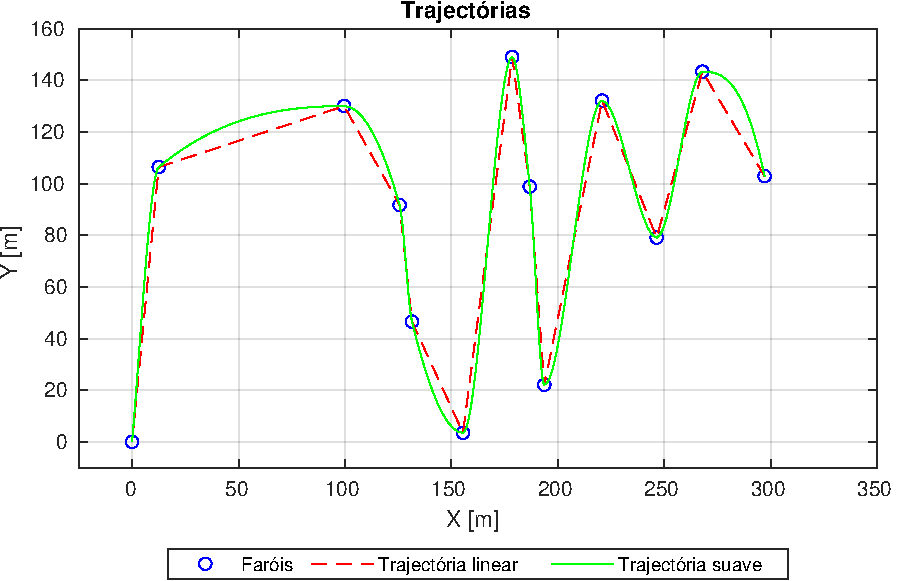
\includegraphics[width=\textwidth]{figs/trajectories.pdf}
         \caption{}
         \label{fig:planning_trajectory}
     \end{subfigure}
     \hfill
     \begin{subfigure}[b]{0.49\textwidth}
         \centering
         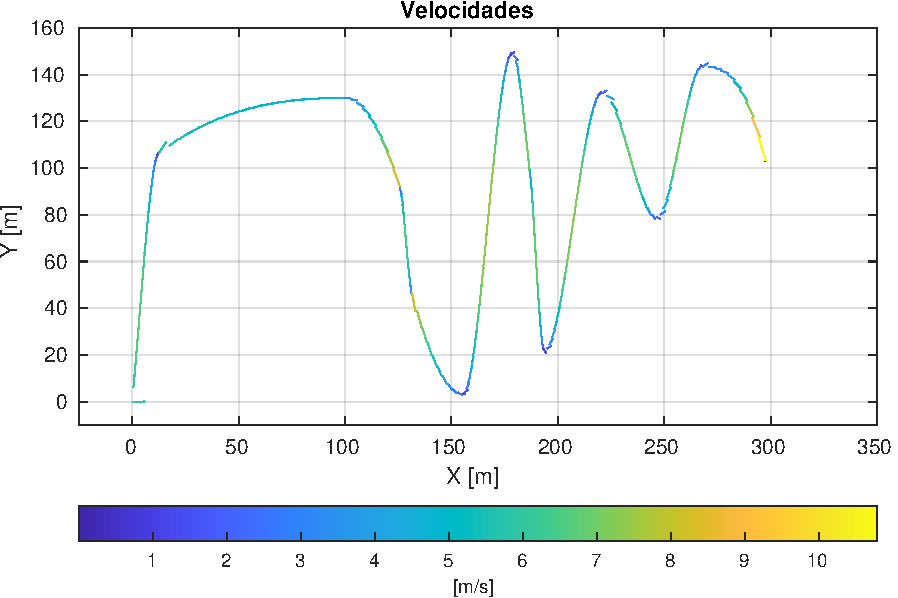
\includegraphics[width=\textwidth]{figs/velocities.pdf}
         \caption{}
         \label{fig:planning_velocities}
     \end{subfigure}
     
     \begin{subfigure}[b]{0.49\textwidth}
         \centering
         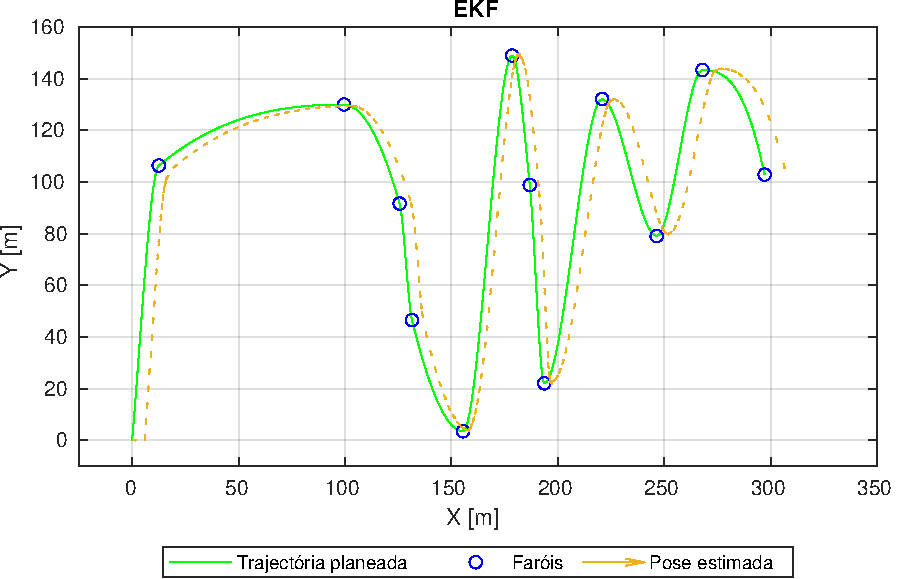
\includegraphics[width=\textwidth]{figs/ekf.pdf}
         \caption{}
         \label{fig:planning_ekf}
     \end{subfigure}
     \hfill
     \begin{subfigure}[b]{0.49\textwidth}
         \centering
         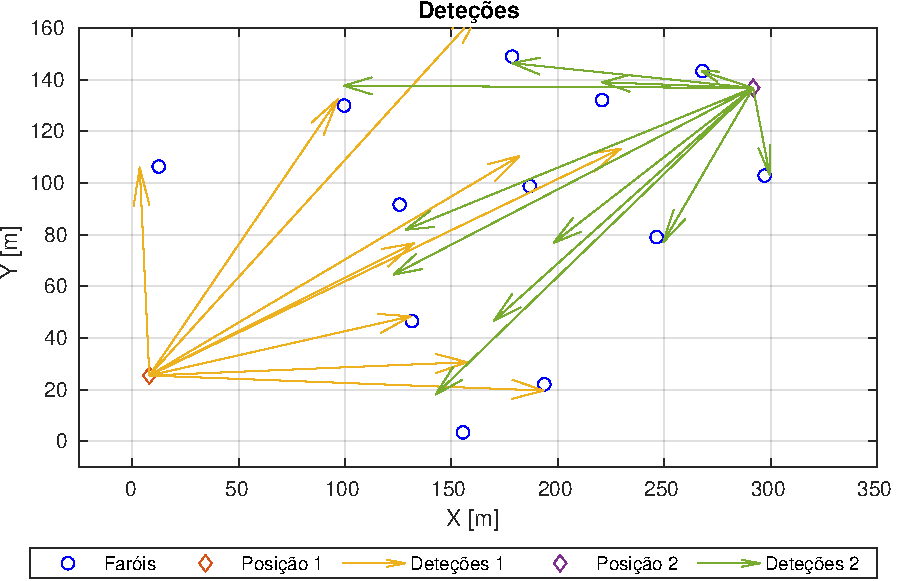
\includegraphics[width=\textwidth]{figs/detections.pdf}
         \caption{}
         \label{fig:planning_detections}
     \end{subfigure}
     
     \begin{subfigure}[b]{0.49\textwidth}
         \centering
         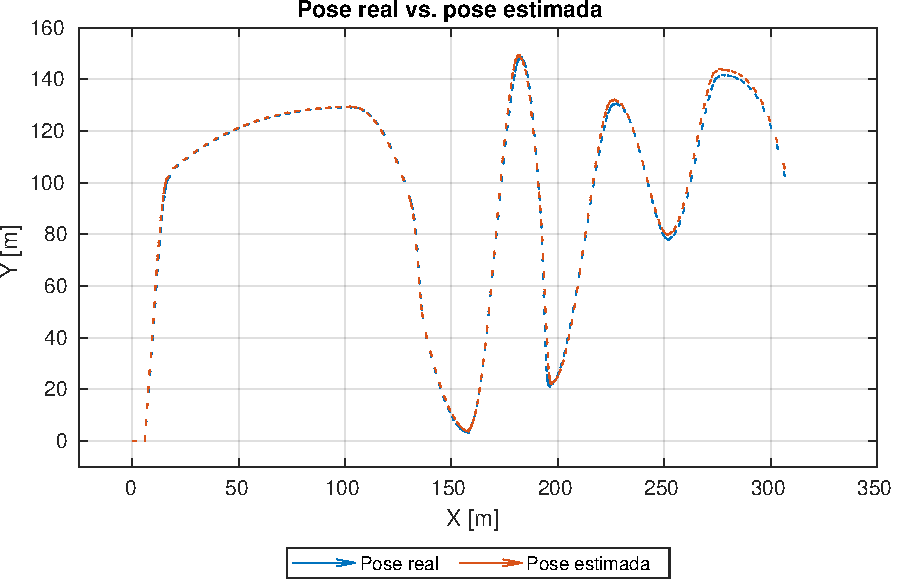
\includegraphics[width=\textwidth]{figs/pose_compare.pdf}
         \caption{}
         \label{fig:ekf_real_compare}
     \end{subfigure}
     \caption{Ilustração do caso de estudo descrito em que se demonstram o trajeto (a) e velocidades (b) planeadas, as sucessivas poses estimadas pelo EKF (c), as deteções dos faróis realizadas pelo robô em duas poses do trajeto (d) e a comparação entre a pose real (com ruído) e a pose estimada pelo EKF (e).}
     \label{fig:planning}
\end{figure}

Para efeitos comparativos, realizou-se o mesmo ensaio anterior, mas aumentando a incerteza na velocidade linear (Fig. \ref{fig:ekf_vn0.1}) ou na velocidade angular (Fig. \ref{fig:ekf_wn0.1}) para 0.1 (na respetiva unidade). Fica assim claro como uma maior incerteza na deteção angular tende a piorar substancialmente os resultados.

\begin{figure}[ht]
     \centering
     \begin{subfigure}[b]{0.49\textwidth}
         \centering
         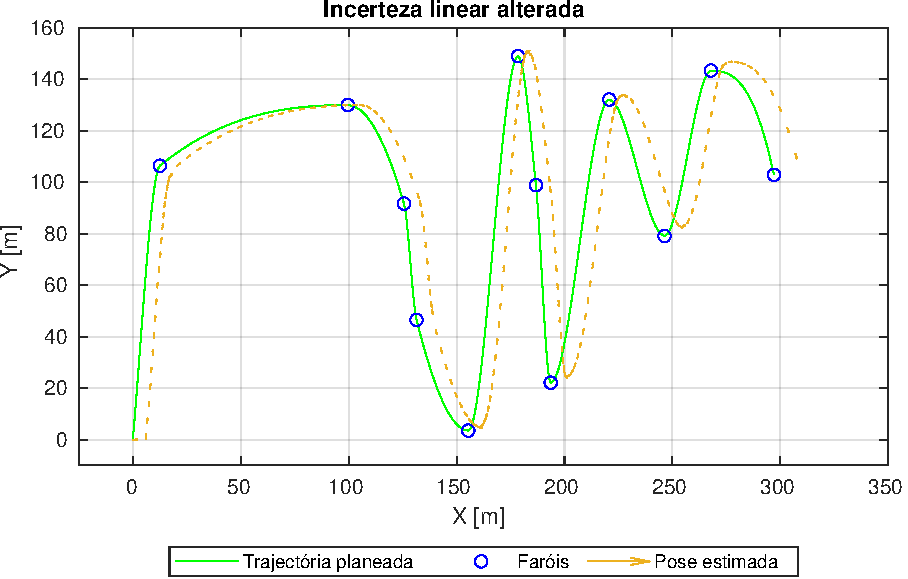
\includegraphics[width=\textwidth]{figs/ekf_vn0.1.pdf}
         \caption{}
         \label{fig:ekf_vn0.1}
     \end{subfigure}
     \hfill
     \begin{subfigure}[b]{0.49\textwidth}
         \centering
         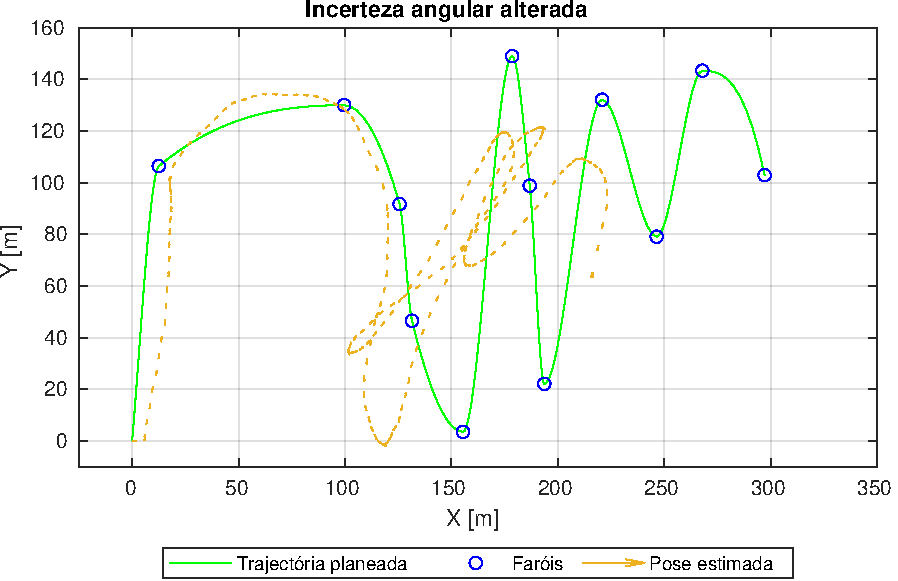
\includegraphics[width=\textwidth]{figs/ekf_wn0.1.pdf}
         \caption{}
         \label{fig:ekf_wn0.1}
     \end{subfigure}
     \caption{Influência da incerteza na velocidade linear (a) e angular (b) nas sucessivas estimativas para a pose.}
     \label{fig:ekf_uncertainty}
\end{figure}

Com o intuito de avaliar eventuais requisitos excessivos aos atuadores dos robôs, a cinemática inversa foi aplicada a cada conjunto de velocidade requisitada. Os resultados demonstrados na Fig. \ref{fig:wheel_speeds} apontam para alguns detalhes importantes.

O modelo com tração diferencial apresenta várias descontinuidades no seu perfil de velocidades (Fig. \ref{fig:diff_wheels}). Estas descontinuidades são principalmente nas localizações dos faróis, onde as curvaturas são mais acentuadas.

Repare-se, ainda, na similaridade entre o perfil de velocidade da roda de tração no triciclo (Fig. \ref{fig:tri_wheels}) com o perfil geral das velocidades na tração diferencial. Esta similaridade existe uma vez que para o modelo utilizado para o triciclo, a roda de tração é na realidade uma roda virtual que acaba por ser a média das rodas esquerda e direita. Ou seja, este triciclo quase que representa um modelo diferencial na traseira responsável apenas pela locomoção ao qual se adiciona uma roda dianteira para impor a orientação.

Já relativamente ao modelo omnidirecional (Fig. \ref{fig:omni_wheels}), este é o único que apresenta velocidades angulares negativas, o que era expectável dado o posicionamento circular das suas rodas e a possível rotação do robô em ambos os sentidos.

\begin{figure}[ht]
     \centering
     \begin{subfigure}[b]{0.49\textwidth}
         \centering
         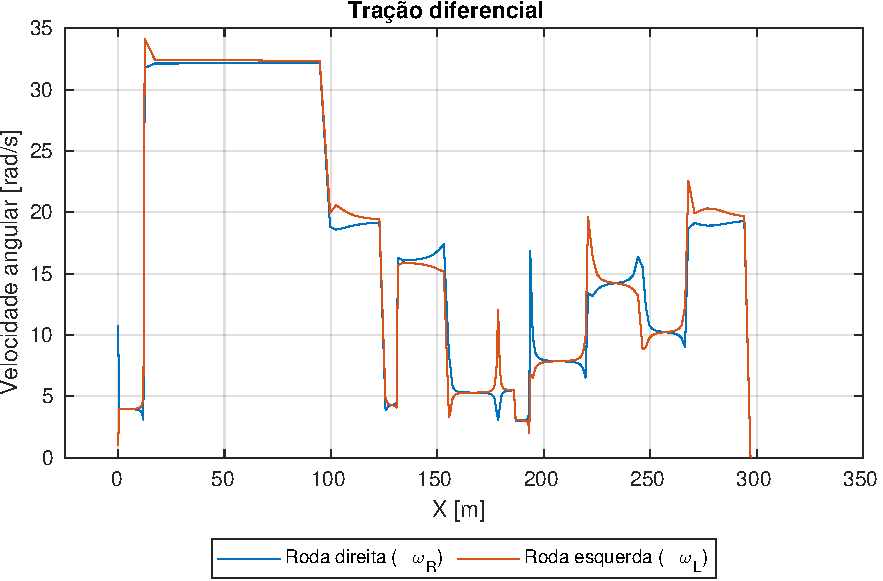
\includegraphics[width=\textwidth]{figs/diff_wheels.pdf}
         \caption{}
         \label{fig:diff_wheels}
     \end{subfigure}
     \hfill
     \begin{subfigure}[b]{0.49\textwidth}
         \centering
         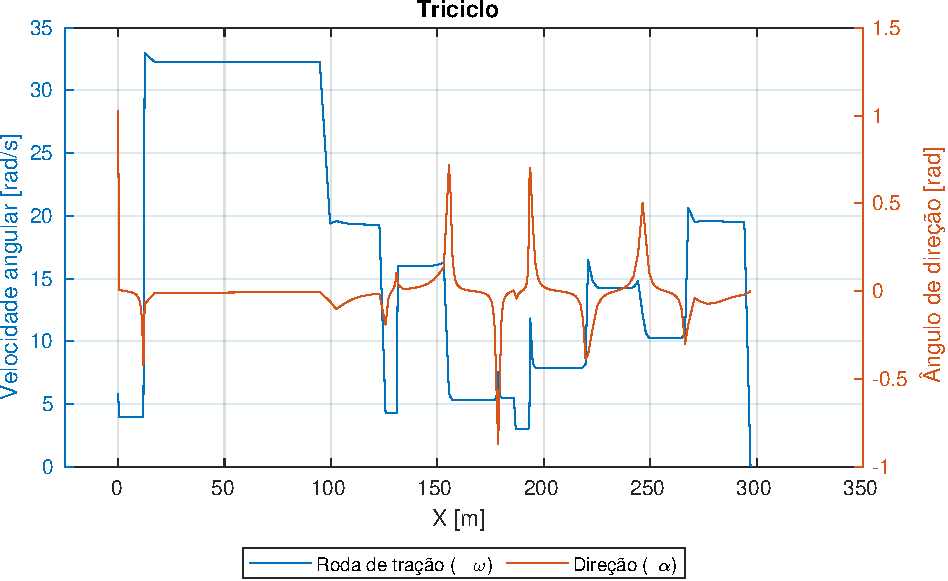
\includegraphics[width=\textwidth]{figs/tri_wheels.pdf}
         \caption{}
         \label{fig:tri_wheels}
     \end{subfigure}
     
     \begin{subfigure}[b]{0.49\textwidth}
         \centering
         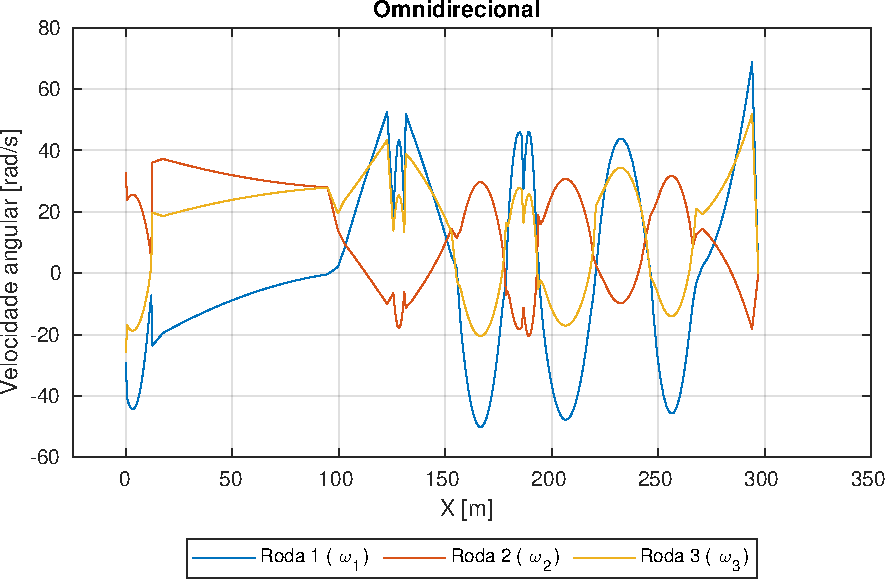
\includegraphics[width=\textwidth]{figs/omni_wheels.pdf}
         \caption{}
         \label{fig:omni_wheels}
     \end{subfigure}
     \caption{Velocidades das rodas dos robôs com tração diferencial (a), triciclo (b) e omnidirecional (c) para o caso de estudo descrito.}
     \label{fig:wheel_speeds}
\end{figure}

\section{Conclusão}

Ficou patente com esta análise a eficácia do filtro de Kalman, em particular na sua versão estendida. Mesmo com observações influenciadas por ruído, assumindo que dentro de limites aceitáveis, o sistema foi capaz de manter uma localização razoável.

A cinemática inversa provou ser a tarefa de maior complexidade devido às complexas equações diferenciais. Graças a ferramentas de calculo simbólico como o \textit{SymPy} ou o próprio \textit{Matlab} e às respetivas restrições impostas, soluções são possíveis de ser definidas e validadas. Ainda assim, e como desenvolvimento futuro, seria interessante estudar o funcionamento de um planeador genérico para tarefas similares às propostas neste projeto.

% \bibliographystyle{abbrv}
% \bibliography{bib}
\printbibliography

\end{document}
